\section{Ray Casting und Ray Tracing}
\label{sec:ray_casting_tracing}

Sofern nicht anders vermerkt, basiert der folgende Abschnitt
auf~\cite{hughes_computer_2013}[Kapitel 15, S. 387ff].

Um ein Bild möglichst realistisch darzustellen muss berechnet werden, wieviel
Licht zu jedem Pixel der sichtbaren Bildfläche (also dem Betrachter)
transportiert wird. Da Photonen die Energie des Lichtes transportieren, muss
man also das physikalische Verhalten dieser simulieren.

Es ist allerdings nicht möglich \textit{alle} Photonen zu simulieren, da
der Aufwand schlicht zu gross wäre. Daher macht es Sinn nur einige
Photonen (exemplarisch) zu betrachten und dann eine Abschätzung des
gesamten Lichtes vorzunehmen.

Jede Lichtquelle emitiert Photonen (als Welle und als Teilchen) in alle
Richtungen. Man modeliert diese als Partikel, welche anhand
Lichtstrahlen (\textit{light rays}) auf Objekte einer
Szene treffen.

Jedes Photon hat dabei eine spezifische Wellenlänge ($\lambda{}$) welche
die Farbe definiert, sowie eine Energie (Frequenz $f$) welche die
Farbintensität des Photons definiert.

Trifft ein Photon auf ein Objekt, wird ein Teil der Energie absorbiert,
ein Teil reflektiert und ein Teil durchdringt das Objekt (Transmission).
Photonen treffen solange auf Objekte bis deren gesamte Energie
absorbiert, sie die Szene verlassen oder sie auf die sichtbare
Bildfĺäche treffen und somit zum eigentlichen Bild beitragen.

Bei Ray Casting bzw. Ray Tracing handelt es sich um eine relativ
einfache Art um globale Beleuchtungsmodelle zu implementieren.

Die einfachste Art Lichtstrahlen zu modellieren ist das so
genannte~\textit{Ray Casting}.

\subsection{Ray Casting}
\label{subsec:ray_casting}

Bei \textit{Ray Casting} handelt es sich um eine Strategie zur
Simulation, wieviel Licht anhand eines (Licht-) Strahles zu der
sichtbaren Bildfläche (also dem Betrachter) transportiert wird.

Das Verfahren wurde erstmals
in~\citetitle{appel_techniques_1968}~\citeyear{appel_techniques_1968}
von~\citeauthor{appel_techniques_1968} vorgeschlagen und
auch~\citeyear{arlington_mathematical_applications_group_inc_afips_1968}
von
der~\citeauthor{arlington_mathematical_applications_group_inc_afips_1968}
in~\citetitle{arlington_mathematical_applications_group_inc_afips_1968}
erfolgreich umgesetzt.

Ein möglicher Algorithmus, wie Ray Casting umgesetzt werden kann, findet
sich in~\autoref{fig:ray_casting:high_level}.

Bei dem Ray Casting Verfahren wird ein \textit{Projektionszentrum} (das
Auge eines Betrachters) sowie eine Region einer beliebigen Bildfläche
gewählt. Dabei kann die Region als gerasterte Fläche angenommen werden.
Jedes Raster entspricht den Bildpunkten (Pixeln) der gewünschten
Auflösung.  Daher, je feiner die Rasterung, desto höher die Auflösung.

Für jeden Bildpunkt der gewählten Region wird ein Strahl
generiert, welcher dann vom Projektionszentrum durch das Zentrum des
Bildpunktes auf die Szene ``geworfen'' wird. 

Es wird dann das Objekt gesucht, welches den nächsten Schnittpunkt mit
dem Strahl bildet. Für jede Lichtquelle der Szene wird geprüft, ob die
Lichtquelle vom Schnittpunkt aus sichtbar ist. Ist dies der Fall, wird
schliesslich die Farbe und die Intensität der Farbe an diesem Schnittpunkt
anhand eines Beleuchtungsmodelles (z.B.\ dem Phong-Beleuchtungsmodell)
berechnet. Ansonsten befindet sich der Punkt im Schatten, wird also
nicht beleuchtet.

\begin{figure}[H]
    \centering
    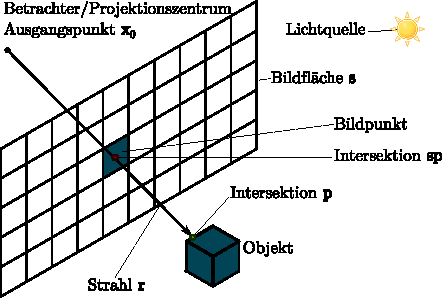
\includegraphics{img/ray_casting.pdf}
    \caption{Illustration des Ray Casting Verfahrens\protect\footnotemark}\label{fig:ray_casting_illustration}
\end{figure}
\footnotetext{Eigene Darstellung mittels Inkscape}

Die obenstehende~\autoref{fig:ray_casting_illustration} zeigt das
Prinzip des Ray Castings. Ausgangspunkt bildet der Betrachter mit $x_{0}
= (x_{x_{0}}, y_{x_{0}}, z_{x_{0}})$. Es wird ein Strahl $r = (x_{0},
d)$ in Richtung $d$ der Bildfläche $s$ ``geworfen''. Der Strahl $r$
schneidet die Bildfläche $s$ an einem Punkt $sp = (x_{sp}, y_{sp},
z_{sp})$.  Somit ergibt sich die Richtung des Strahles $d = sp - x_{0} =
(x_{sp} - x_{x_{0}}, y_{sp} - y_{x_{0}}, z_{sp} - z_{x_{0}}) = (x_{d},
y_{d}, z_{d})$. Der Strahl $r$ trifft und schneidet schliesslich ein
Objekt am Punkt $p = r(t) = x_{0} + t \cdot d$ wobei $t \in [1, \infty]$
ist. Dies führt dazu, dass das Raster respektive der Bildpunkt, durch
welches der Strahl $r$ hindurch geht, die Farbe des getroffenen Objektes
annimmt.

\subsubsection{Berechnung von Schnittpunkten}
\label{ssubsec:ray_casting_intersections}

Um den Schnittpunkt eines Lichtstrahles mit einem Objekt zu berechnen
wird grundsätzlich die mathematische Gleichung des Lichtstrahles in die
des Objektes eingesetzt. Existiert eine reelle Lösung, so schneidet der
Lichtstrahl das Objekt am nächsten Punkt zwischen dem Schnittpunkt und
der Oberflächennormale des Objektes.

~\citeauthor{glassner_introduction_1989} beschreibt mehrere Methoden zur
Prüfung von Schnittpunkten, hier sei beispielhalber nur die Intersektion
mit einer Kugel sowie mit einem Dreieck genannt.

\textit{Schnittpunkt mit einer Kugel}

Um den Schnittpunkt bzw.\ die Schnittpunkte eines Lichtstrahles mit
einer Kugel zu erhalten, wird die Gleichung des Lichtstrahles

\begin{gather}\label{eq:ray_equation}
    r(t) = r_{0} + t \cdot r_{d}
\end{gather}

in die implizite Gleichung einer Kugel

\begin{gather}
    \|\bm{x} - c\|^{2} - r^{2} = 0
\end{gather}

eingesetzt. Dies führt zu folgendem Gleichungssystem:

\begin{align}
    \|r(t) - c\|^{2} - r^{2} &= 0 \\
    \|r_{0} + t \cdot r_{d} - c\|^{2} - r^{2} &= 0
\end{align}

Das Auflösen dieses Gleichungssystemes ergibt folgende Fälle:

\begin{itemize}
    \item{Zwei Lösungen}: Der Strahl geht durch die Kugel hindurch.
    \item{Eine Lösungen}: Der Strahl streift die Kugel an einem Punkt
        als Tangente.
    \item{Imaginäre Lösung}: Der Strahl verfehlt die Kugel komplett.
\end{itemize}


\textit{Schnittpunkt mit einem Dreieck}

Um den Schnittpunkt eines Lichtstrahles mit einem Dreieck zu erhalten,
wird die Gleichung des Lichtstrahles~\ref{eq:ray_equation} als Lösung
der Gleichung eines Dreiecks mit baryzentrischen Koordinaten

\begin{gather}
    x(\beta, \gamma) = v_{1} + \beta(v_{2} - v_{1}) + \gamma(v_{3} - v_{1})
\end{gather}

verwendet. Dies führt zu folgendem Gleichungssystem:

\begin{align}
    r_{0} + t \cdot r_{d} &= v_{1} + \beta(v_{2} - v_{1}) + \gamma(v_{3} - v_{1})
\end{align}

Der Lichtstrahl schneidet das Dreieck genau dann, wenn gilt $\beta +
\gamma \le 1$, $\beta \ge 0$ und $\gamma \ge 0$.

Es ist leicht verständlich, dass es sehr aufwändig ist jegliche Objekte
auf Schnittpunkte zu testen (so wie in
Beispiel~\ref{fig:ray_casting:high_level}). So wurde eine Vielzahl an
Methoden entwickelt um dies zu Beschleunigen. Eine Möglichkeit ist es,
das Finden der Schnittpunkte zu Beschleunigen, z.B. durch Verwendung von
Hüllköpern, oder die Anzahl der Berechnungen zu minimieren, z.B. durch
Verwendung von Hierarchien von Objekten oder der Unterteilung des Raumes
einer Szene. Das Kapitel ``A Survey of Ray Tracing Accelelration
Techiques'' von~\citeauthor{glassner_introduction_1989} in~\citetitle[S.
202ff]{glassner_introduction_1989}, bietet einen guten Überblick.

\begin{lstlisting}[language=Python,caption={Eine abstrakte Umsetzung des Ray
        Casting Verfahrens\protect\footnotemark.},label={fig:ray_casting:high_level},captionpos=b,emph={ray_cast}]
def ray_cast():
    # "pixels" is a list of all pixels of the image plane
    for pixel in pixels:
        # Save all intersections for given pixel
        intersections = []

        # Returns the ray passing through the given
        # pixel from the eye
        ray = ray_at_pixel(pixel)

        # "scene_triangles" is a list of all triangles
        # coming from meshes contained in the scene to render
        for triangle in scene_triangles:
            p   = intersect(ray, triangle)
            sum = 0

            for light in incoming_lights_at_p:
                sum = sum + l.value
            end

            if is_smallest_intersection(p, intersections):
                pixel = sum
            intersections.append(p)
\end{lstlisting}
\footnotetext{Algorithmus in Pseudocode gemäss~\cite[Kapitel 15, Seite 391, Auflistung 15.2]{hughes_computer_2013}}

\subsection{Ray Tracing}
\label{subsec:ray_tracing}

Sofern nicht anders vermerkt, basiert der folgende Abschnitt
auf~\cite{glassner_introduction_1989}[S. 1 bis 77].

Bei dem heute als Ray Tracing bekannten Verfahren, handelt es sich um
eine verbesserte Version des unter~\ref{subsec:ray_casting} genannten
Ray Casting Verfahrens. \citeauthor{whitted_improved_1980} publizierte
das Verfahren~\citeyear{whitted_improved_1980} im Paper
``\citetitle{whitted_improved_1980}''.

Ein möglicher Algorithmus, wie Ray Tracing umgesetzt werden kann,
findet sich in~\ref{fig:ray_tracing:high_level}.

Grundsätzlich ist die Idee, dass jeder Bildpunkt der gewählten Region
Licht aus nur einer Richtung erhält --- der Richtung der Lichtstrahlen
(\textit{light rays}), welche durch die gewählte Region und die
sichtbare Bildfläche gehen. Somit trägt jedes Photon, welches aus dieser
Richtung kommt, zum Farbwert bzw.\ der Intensität der Farbe eines
Bildpunktes bei. Bei Strahlen, welche das Licht direkt zur sichtbaren
Bildfläche transportieren, spricht man von \textit{Pixel}- bzw.\
\textit{Augen-Strahlen}.~\cite{glassner_introduction_1989}[S. 10]

\begin{figure}[H]\label{fig:ray_tracing_scene}
    \centering
    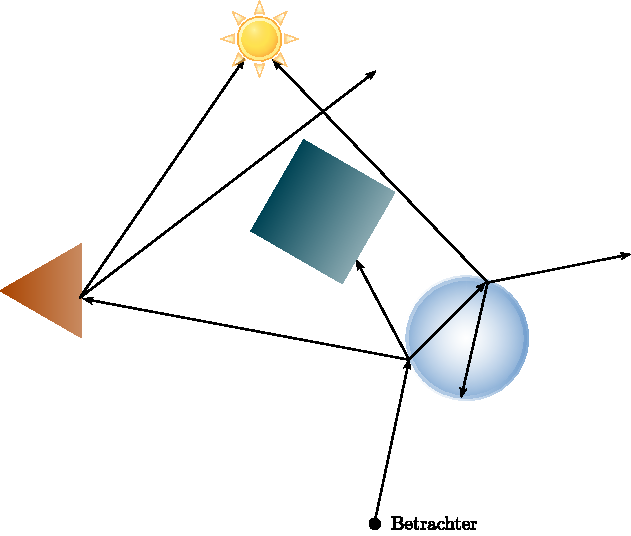
\includegraphics{img/ray_tracing_scene.pdf}
    \caption{Illustration des Ray Tracing Verfahrens\protect\footnotemark}
\end{figure}
\footnotetext{Eigene Darstellung mittels Inkscape angelehnt
    an~\cite{glassner_introduction_1989}[S. 16]}

Die Strahlen werden in dieser Richtung verfolgt, um festzustellen wie
das Licht ``erzeugt'' wird. Trifft der Strahl auf nichts wird die
Verfolgung des Strahles beendet und der Bildpunkt wird mit der Farbe des
Hintergrundes eingefärbt. Trifft der Strahl direkt auf eine Lichtquelle
wird die Verfolgung des Strahles beendet und der Bildpunkt wird mit der
Farbe und Intensität der Lichtquelle eingefärbt.  Trifft der Lichtstrahl
auf eine Oberfläche, wird der Prozess von diesem Punkt aus neu gestartet
um festzustellen, wie das Licht dort ``erzeugt'' wurde. 

Wie der letzte Punkt zeigt, handelt es sich um ein rekursives Verfahren
und wird daher teilweise auch rekursives Ray Tracing genannt.

Zur Berechnung des emittierten Lichtes an einem gewissen Punkt auf der
Oberfläche eines Objektes, wird in einem ersten Schritt die Intensität
des Lichtes dieses Punktes bestimmt. Man spricht dabei von \textit{Licht}- bzw.\
\textit{Schatten-Strahlen}.~\cite{glassner_introduction_1989}[S. 10]

In einem weiteren Schritt wird berechnet, wie die Oberfläche an
diesem Punkt Licht in eine spezifische Richtung weitergibt. Dies
geschieht durch die Intensität des Lichtes des Punktes sowie dessen
physikalischen Eigenschaften.

Trifft ein Lichtstrahl auf eine Oberfläche, wird dieses zu gewissen
Teilen~\textit{absorbiert}, \textit{reflektiert} und
\textit{gebrochen}.Die jeweiligen Anteile hängen dabei vom Medium der
Oberfläche bzw.\ des Objektes, der Frequenz des Lichtes sowie zwischen
dem eingehenden Winkel des Lichtstrahles und der Oberflächennormale ab.
Licht kann je nach Medium auch gestreut werden.

Man unterscheidet zwischen vier verschiedenen Mechanismen wie Licht
transportiert wird: Perfekt diffuse, perfekt spiegelnde, perfekt
brechende und total interne
Reflexion.~\cite{glassner_introduction_1989}[S. 130 bis 137]
In der Realität bzw.\ der Natur kann es sein, dass mehrere der
Mechanismen gemischt auftreten. So wird z.B.\ ein Teil des Lichtes
reflektiert, wohingegen ein anderer Teil das Objekt durchdringt.

Die von diesen Mechanismen emittierten Strahlen können
gemäss~\citeauthor{glassner_introduction_1989}
in~\textit{Reflexion-Strahlen}, welche die perfekte diffuse und die
perfekt spiegelnde Reflexion beschreiben,
und~\textit{Transparenz-Strahlen}, welche die perfekt brechende und die
totale interne Reflexion beschreiben,unterteilt
werden.~\cite{glassner_introduction_1989}[S. 10]

\begin{figure}[H]\label{fig:ray_tracing_scene_rays}
    \centering
    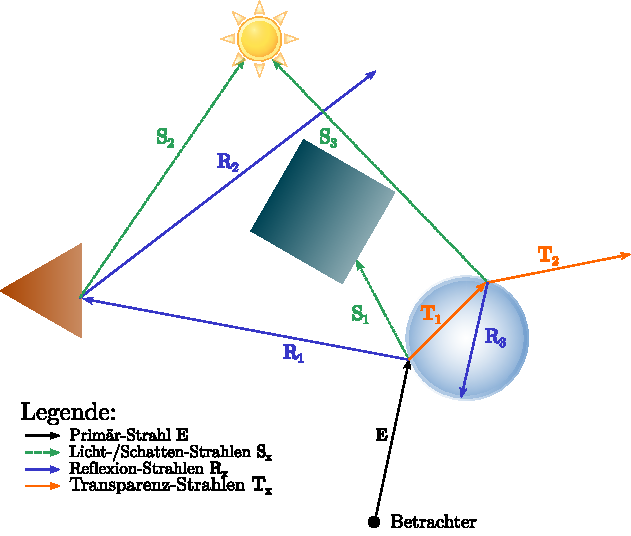
\includegraphics{img/ray_tracing_scene_rays.pdf}
    \caption{Illustration der einzelnen Strahlen und deren Verhalten
        ausgehend von der Szene in
        Abbildung.~\ref{fig:ray_tracing_scene}\protect\footnotemark{}
        Das im Bild ersichtliche, orange-farbige Dreieck hat eine
        undurchlässige, reflexive Oberfläche. Der türkis-farbige Würfel
        hat eine diffuse Oberfläche.  Bei der Kugel, rechts im Bild,
        handelt es sich um eine Kugel aus Glas, welche das Licht
        teilweise bricht und reflektiert.}
\end{figure}

\footnotetext{Eigene Darstellung mittels Inkscape angelehnt
    an~\cite{glassner_introduction_1989}[S. 16]}

Nachfolgend werden die oben genannten Strahlen im Einzelnen beschrieben.

\subsubsection{Augen- oder Pixel-Strahlen}
\label{ssubsec:ray_tracing:eye_rays}

Augen- oder Pixel-Strahlen sind Strahlen, welche das Licht von einer
Lichtquelle durch einen Bildpunkt direkt zu der sichtbaren Bildfläche
(also dem Betrachter) transportieren.

Die Gleichung solcher Strahlen lautet:

\begin{gather}
    r(t) = x_{0} + t \cdot (S - x_{0})
\end{gather}

Wobei $x_{0}$ der Ausgangspunkt (also der Betrachter), $t$ ein
Skalierungsfaktor zwischen $[1, \infty]$ und $S$ der Schnittpunkt mit der
Bildfläche ist.

\subsubsection{Licht- oder Schatten-Strahlen}
\label{ssubsec:ray_tracing:shadow_rays}
Bei Licht- bzw.\ Schatten-Strahlen handelt es sich um Strahlen, welche
das Licht von einer Lichtquelle direkt zu der Oberfläche eines
Objektes transportieren. Bei jedem Schnittpunkt eines Primär-Strahles
(also ein Strahl welcher vom Betrachter aus in die Szene ``geworfen''
wird) mit einem Objekt wird ein Schatten- bzw.\ Licht-Strahl in Richtung jeder
Lichtquelle der Szene ``geworfen''. Trifft der Schatten- bzw.\
Licht-Strahl die Lichtquelle, wird das Licht zur Berechnung der Farbe
und Intensität des Lichtes genutzt. Trifft der Schatten-Strahl keine
Lichtquelle, so wird das Licht nicht berücksichtigt. Schatten-Strahlen
generieren keine weiteren Strahlen.

Die Gleichung von Licht- bzw.\ Schatten-Strahlen lautet:

\begin{gather}
    r(t) = p_{0} + t \cdot (L_{i} - p_{0})
\end{gather}

Wobei $p_{0}$ der Ausgangspunkt (also ein Punkt auf einer Oberfläche
eines Objektes), $t$ ein Skalierungsfaktor zwischen $[\epsilon, 1]$ und
$L_{i}$ der Ort der $i$-ten Lichtquelle ist. Bei $\epsilon$ handelt es
sich um einen Faktor zur Steuerung der Präzision, welcher verhindert,
dass ein Objekt lokal auf sich selbst Schatten wirft.


\subsubsection{Reflexion-Strahlen}
\label{ssubsec:ray_tracing:reflection_rays}

Die Eigenschaften von Licht, welches auf ein Objekt trifft und dann an
diesem gespiegelt wird, werden durch~\textit{Reflexion-Strahlen}
bestimmt. Wie bereits vorhergehend beschrieben, gibt es zwei Arten der
Reflexion: Perfekt diffuse und perfekt spiegelnde Reflexion.

\textbf{Perfekt spiegelnde Reflexion}

Bei der perfekt spiegelnden Reflexion verlässt der ausgehende Strahl die
Oberfläche in demselben Winkel wie der eingehende Strahl hat. Der
Ausfallswinkel entspricht also dem Einfallswinkel.

Die Gleichung eines von einer perfekt spiegelnden Reflexion ausgehenden
Strahles lautet~\cite{glassner_introduction_1989}[S. 132]:

\begin{align}
    r(t) &= p_{0} + t \cdot R \\
    R &= I - 2(I \cdot N)N
\end{align}

Wobei $p_{0}$ der Ausgangspunkt (also ein Punkt auf einer Oberfläche
eines Objektes), $t$ ein Skalierungsfaktor zwischen $[\epsilon, 1]$, $I$
der eingehende Vektor, also $S - x_{0}$, und $N$ die Oberflächennormale
ist. Bei Epsilon handelt es sich wiederum um einen Faktor zur Steuerung
der Präzision, welcher verhindert, dass ein Objekt lokal in sich selbst
gespiegelt wird.

\begin{figure}[H]\label{fig:ray_tracing_specular_reflection}
    \centering
    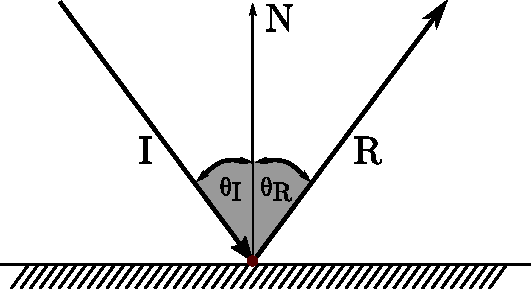
\includegraphics{img/perfect_specular_reflection.pdf}
    \caption{Illustration einer perfekt spiegelnden
        Reflexion.~\protect\footnotemark{}
        $I$ ist der eingehende Strahl, welcher am Normalenvektor $N$ der
        schraffierten Oberfläche in Richtung $R$ reflektiert wird. Der
        Winkel des eingehenden Strahles $\theta_{I}$ ist gleichgross wie der
        Winkel des ausgehenden Strahles $\theta_{R}$.}
\end{figure}
\footnotetext{Eigene Darstellung mittels Inkscape angelehnt
    an~\cite{glassner_introduction_1989}[S. 131]}


\textbf{Perfekt diffuse Reflexion}

Bei der perfekt diffusen Reflexion wird das eingehende Licht mit
gleicher Amplitude (also Stärke) gleichmässig in alle Richtungen
gestreut. Die Amplitude ist dabei proportional zum Kosinus des
Einfallswinkels und der Oberflächennormale.

\begin{figure}[H]\label{fig:ray_tracing_diffuse_reflection}
    \centering
    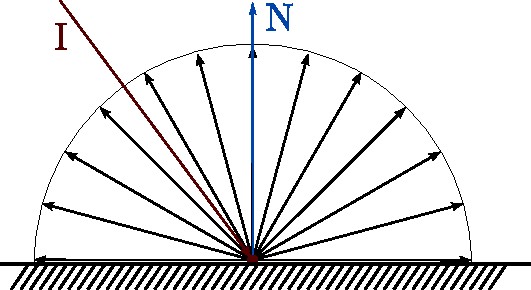
\includegraphics{img/perfect_diffuse_reflection.pdf}
    \caption{Illustration einer perfekt diffusen
        Reflexion.~\protect\footnotemark{}
        $I$ ist der eingehende Strahl, welcher am Ort des
        Normalenvektors $N$ der schraffierten Oberfläche auftrifft. Das
        Licht wird gleichmässig in alle Richtungen gestreut.}
\end{figure}
\footnotetext{Eigene Darstellung mittels Inkscape angelehnt
    an~\cite{glassner_introduction_1989}[S. 134]}

\subsubsection{Transparenz-Strahlen}
\label{ssubsec:ray_tracing:transparency_rays}

Und schliesslich werden die Eigenschaften von Licht, welches durch ein
Objekt hindurch geht und vielleicht von diesem gebrochen wird, durch
die~\textit{Transparenz-Strahlen} beschrieben.  Auch hier werden zwei
Arten der Reflexion unterschieden: Perfekt brechende und total interne
Reflexion.

\textbf{Perfekt brechende Reflexion}

Tritt Licht von einem Medium (z.B.\ Luft) in ein anderes Medium (z.B.\
Glas) ein, so wird das Licht umgelenkt. Die Umlenkung des Lichtes bei
Eintritt in ein neues Medium wird auch Transmission oder Refraktion
genannt. Jedes Medium hat dabei einen eignen Index der Refraktion,
welcher Lichtgeschwindigkeit in dem Medium gegenüber
Lichtgeschwindigkeit im Vakuum beschreibt.
Um zu entscheiden wie Licht umgelenkt wird, werden die
Refraktion-Indizes der Medien sowie der Einfalls- bzw. Ausfallswinkel
verglichen.

Die Beziehung zwischen dem Einfalls- und Ausfallswinkel sowie dem
übertragenen Licht wird durch das Gesetz von ``Snell'' beschrieben:

\begin{gather}
    \frac{\sin(\theta_{1})}{\sin(\theta_{2})} = \eta_{21} = \frac{\eta_{2}}{\eta_{1}}
\end{gather}

Wobei $\theta_{1}$ der Einfallswinkel der Einfallswinkel, $\theta_{2}$
der Ausfallswinkel, $\eta_{1}$ der Refraktion-Index des ersten Mediums
in Abhängigkeit zum Vakuum, $\eta_{2}$ der Refraktion-Index des zweiten
Mediums in Abhängigkeit zum Vakuum und $\eta_{21}$ der Refraktion-Index
des zweiten Mediums in Abhängigkeit zu dem ersten Medium
ist.~\cite{glassner_introduction_1989}[S. 134 bis 135]

Umgekehrt kann das Verhältnis des ausgehenden Strahles zum eingehenden
Strahl beschreiben werden:

\begin{gather}
    \eta_{12} = \frac{\eta_{1}}{\eta_{2}} = \frac{\sin(\eta_{2})}{\sin(\eta_{1})}
\end{gather}

Mithilfe dieses Verhältnisses kann der gebrochene Strahl wie folgt
berechnet werden~\cite{glassner_introduction_1989}[S. 137 bis 140]:

\begin{align}
    r(t) &= p_{0} + t \cdot T \\
    T &= \eta_{12}I + (\eta_{12} \cdot C_{1} - \sqrt{C_{2}})N
    \label{eq:ray_tracing:transm} \\
    C_{1} &= -I \cdot N \\
    C_{2} &= 1 + \eta_{12}^{2}(C_{1}^{2} - 1) \label{eq:ray_tracing:transm_c2}
\end{align}

Wobei $p_{0}$ der Ausgangspunkt (also ein Punkt auf einer Oberfläche
eines Objektes), $t$ ein Skalierungsfaktor zwischen $[\epsilon, 1]$, $I$
der eingehende Vektor, also $S - x_{0}$, $N$ die Oberflächennormale und
$\eta_{12}$ das oben beschriebene Verhältnis ist.
Bei Epsilon handelt es sich wiederum um einen Faktor zur Steuerung
der Präzision, welcher verhindert, dass ein Objekt lokal in sich selbst
gespiegelt wird.

\begin{figure}[H]\label{fig:ray_tracing_specular_transmission}
    \centering
    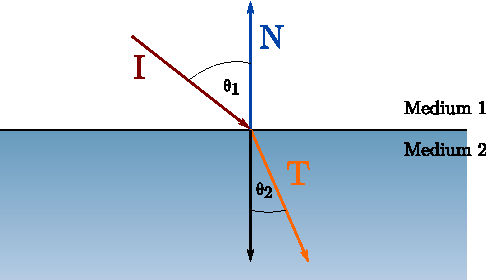
\includegraphics{img/perfect_specular_tranmission.pdf}
    \caption{Illustration einer perfekt brechenden
        Reflexion.~\protect\footnotemark{}
        $I$ ist der eingehende Strahl, welcher am Ort des
        Normalenvektors $N$ im Winkel von $\theta_{1}$ von Medium 1 in
        Medium 2 übergeht und entsprechend mit Winkel $\theta_{2}$
        anhand $T$ gebrochen wird.}
\end{figure}
\footnotetext{Eigene Darstellung mittels Inkscape angelehnt
    an~\cite{glassner_introduction_1989}[S. 135]}

\textbf{Totale interne Reflexion}

Die totale interne Reflexion tritt dann auf, wenn Licht unter einem zu
flachen Winkel versucht von einem dichten Medium in ein weniger dichtes
Medium zu gelangen. Das Licht prallt am Übergang der beiden Medien ab
und wird gespiegelt anstatt in das andere Medium
einzutreten.~\cite{glassner_introduction_1989}[S. 136 bis 137]

Dies geschieht dann, wenn der Term $C_{2}$
(Gleichung~\ref{eq:ray_tracing:transm_c2}) negativ ist und somit das
Ergebnis der Wurzel aus $C_{2}$ in~\ref{eq:ray_tracing:transm} eine
imaginäre Zahl wird.~\cite{glassner_introduction_1989}[S. 137 bis 138]

\begin{figure}[H]\label{fig:ray_tracing_total_internal_reflection}
    \centering
    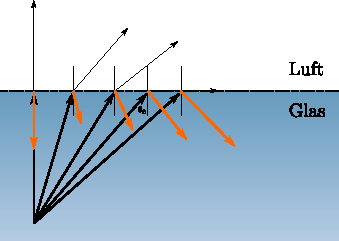
\includegraphics{img/total_internal_reflection.pdf}
    \caption{Illustration der totalen internen
        Reflexion.~\protect\footnotemark{}
        Ist der kritische Winkel $\theta_{c}$ beim Übertritt eines
        Strahles von einem Medium (hier Glas) zu einem anderen Medium (hier
        Luft) nicht überschritten, so wird der Strahl bzw.\ Licht sowohl
        gebrochen als auch reflektiert. Wird der kritische Winkel
        überschritten, so findet nur noch eine Reflexion
        statt.\protect\footnotemark}
\end{figure}
\footnotetext{Eigene Darstellung mittels Inkscape angelehnt
    an~\cite{glassner_introduction_1989}[S. 137]}
\footnotetext{\cite{glassner_introduction_1989}[S. 137]}

\subsubsection{Modelle zur Schattierung (shading models)}
\label{ssubsec:ray_tracing:shading_models}

\citeauthor{glassner_introduction_1989} beschreibt auf der Physik
basierende Modelle zur Schattierung (shading models, welche heute unter
dem Begriff PBRT --- Physically Based Rendering bekannt sind). Diese
hier aufzuführen würden den Rahmen dieser Projektarbeit sprengen, daher
wird darauf verzichtet. Dem geneigten Leser sei
auf~\citetitle{glassner_introduction_1989}[S. 143ff]
sowie~\citetitle{pharr_physically_2010} empfohlen.

\subsubsection{Rekursion und Strahlen-Baum}
\label{ssubsec:ray_tracing:recursion}

Sofern nicht anders vermerkt, basiert der folgende Abschnitt
auf~\cite{glassner_introduction_1989}[S. 16 bis 17].

Wie zu Beginn des Kapitels bereits angesprochen wurde, handelt es sich
bei Ray Tracing um ein rekursives Verfahren. Es stellt sich somit die
Frage, wie tief die Rekursion gehen soll und auch kann.\\
Zusätzlich zu dem genannten Fall, dass ein Strahl auf kein Objekt
innerhalb der Szene trifft, schlagen~\citeauthor{whitted_improved_1980}
wie auch~\citeauthor{glassner_introduction_1989} den Abbruch in
folgenden Fällen vor:
\begin{itemize}
        \item{Nach Erreichen einer festgelegten, maximalen Tiefe},
            sofern die Rekursion rein auf reflexive Oberflächen trifft.
        \item{Nach dem Auftreffen auf eine rein diffuse Oberfläche.}
        \item{Nach Unterschreiten eines minimalen Energiewertes des
                Lichtes.}
\end{itemize}

Aus den genannten Abbruch-Kriterien ergibt sich folgende
nach~\citeauthor{heckbert_adaptive_1990} folgende, auf einem regulären
Ausdruck basierende Lichtweg-Notation: \textbf{LD?S*E}. Diese beschreibt den
Weg, welchen ein Photon ausgehend von einer Lichtquelle (\textbf{L}) zum Auge eines
Betrachters (\textbf{E}) nehmen kann. Es kann auf null oder genau eine diffuse
Oberfläche (\textbf{D?}) so wie auf 0 oder theoretisch unendlich viele reflektierende
Oberflächen (\textbf{S*}) treffen.~\cite{heckbert_adaptive_1990}[S. 148]

Ausgehend von der sichtbaren Bildfläche, also dem Auge des Betrachters
der Szene, kann so ein Strahlen-Baum (\textit{ray tree}) aufgebaut
werden.

Jeder Schnittpunkt eines Strahles mit einem Objekt kann
Sekundär-Strahlen generieren und so bilden reflektierte und gebrochene
Strahlen den Strahlen-Baum.

Dabei sind die \textit{Knoten} des Baumes die Schnittpunkte und die
\textit{Kanten} sind die reflektierten oder gebrochenen Strahlen.

Wie bereits erwähnt wird bei jedem Schnittpunkt ein Schatten-Strahl
ausgesendet, welcher aber keine zusätzlichen Strahlen und somit auch
keine zusätzlichen Kanten generiert.

Der Strahlen-Baum kann so schliesslich von unten nach oben
(\textit{bottom-up}) traversiert werden, was einer Tiefensuche
(depth-first traversal) entspricht. Die Farbe eines Knoten wird aufgrund
der Farbe der Kindes-Knoten berechnet.

\begin{table}[H]
    \centering
    \caption{Darstellung des Strahlen-Baumes anhand einer
        Beispielszene}\label{table:ray_tracing:ray_tree}
    \begin{tabular}{p{0.3\textwidth}p{0.3\textwidth}p{0.3\textwidth}}
        \toprule
            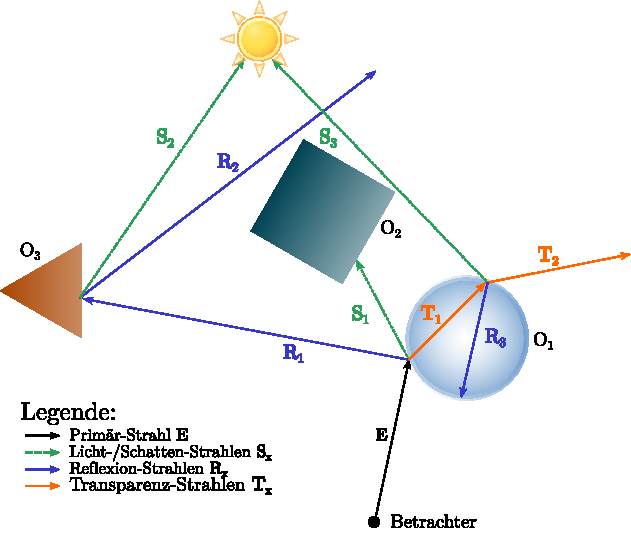
\includegraphics[width=0.3\textwidth]{img/ray_tracing_scene_ray_tree.pdf} &
            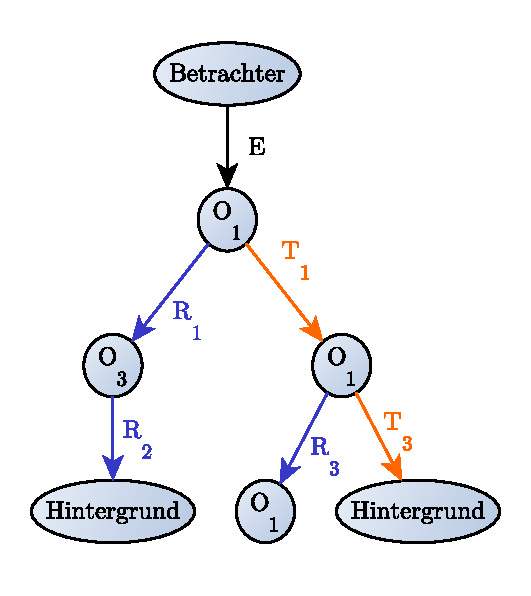
\includegraphics[width=0.3\textwidth]{img/ray_tracing_tree.pdf} &
            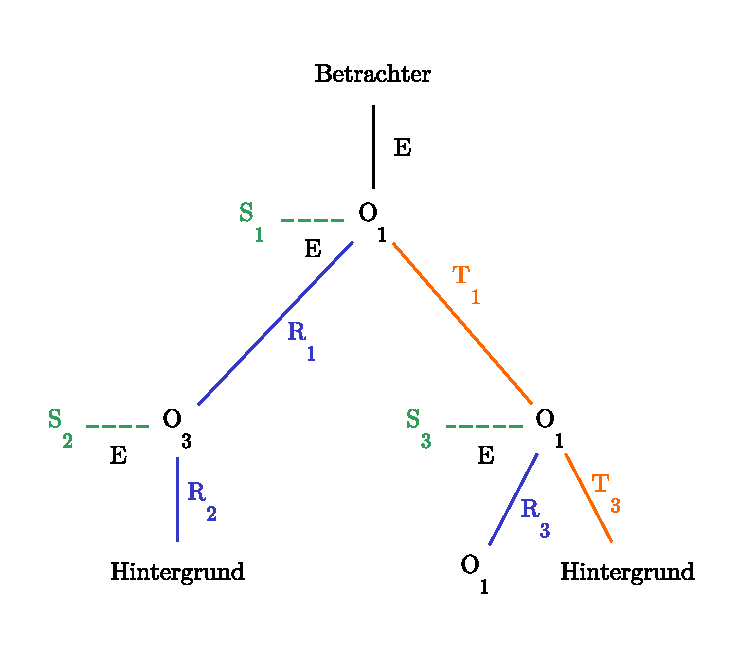
\includegraphics[width=0.3\textwidth]{img/ray_tracing_tree_schematic.pdf} \\
            Beispielszene &
            Gerichteter Strahlen-Baum &
            Schematischer Strahlen-Baum
            nach~\citeauthor{glassner_introduction_1989} \\
        \bottomrule
    \end{tabular}
\end{table}

\begin{lstlisting}[language=Python,caption={Eine abstrakte Umsetzung des
        Ray Tracings \protect\footnotemark.},
    label={fig:ray_tracing:high_level},captionpos=b,emph={ray_trace}]
def ray_trace(current_point, direction):
"""Traces light rays from current point in space in given direction.

:param current_point: current point in space
:type  current_point: three dimensional point object
:param direction:     the direction to trace
:type  direction:     three dimensional vector

:return:              the color for the given point
:rtype:               float
"""

    # Set color to currently set background color
    color = self.background_color

    # "pixels" is a list of all pixels of the image plane
    for pixel in pixels:

        # Returns the ray passing through the given
        # pixel from the eye
        ray = ray_at_pixel(pixel)

        # object_list is a list containing all the meshes contained in
        # the scene to render
        for object in object_list:
            p = intersect(ray, object)

            if object.is_reflective:
                reflection_vector = reflect(direction, object)
                reflected_color   = ray_trace(p, reflection_vector)
                color = color + object.coeff * reflected_color

            if object.is_refractive:
                refracted_vector = refract(direction, object)
                refracted_color  = ray_trace(p, refracted_vector)
                color = color + object.coeff * refracted_color

            for light in incoming_lights_at(p):
                if not is_shadow_ray(p, light.position):
                    color = color + calc_lighting(p, direction, light, object)
            end
        end
    end

    return color
end
\end{lstlisting}
\footnotetext{Algorithmus in Pseudocode
    gemäss~\cite{glassner_introduction_1989}[Seite 283]}

